\documentclass[fleqn,10pt]{olplainarticle}
% Use option lineno for line numbers 

\title{Data Quality Assessment and Periodicity Analysis of Old Faithful Geyser Eruption Patterns}

\author[1]{Lauhitya Reddy}
\affil[1]{Department of Biomedical Informatics, Emory University}

\usepackage{graphicx}
\usepackage{booktabs}

\begin{document}

\flushbottom
\maketitle
\thispagestyle{empty}

\begin{abstract}
This study presents a comprehensive data quality assessment and preprocessing pipeline for the Old Faithful geyser dataset, followed by a novel periodicity analysis of eruption patterns. We systematically addressed data quality issues including malformed entries, alphanumeric contamination, and logical inconsistencies, achieving a 98.2\% retention rate (267 of 272 samples). Our analysis reveals distinct proportional relationships between eruption duration and waiting time within individual cycles, with an average eruption duration comprising 35.8\% of the total cycle time. The developed pipeline demonstrates robust preprocessing capabilities while the ring visualization effectively illustrates the cyclical nature of geyser behavior.
\end{abstract}

\section*{Introduction}

The Old Faithful geyser in Yellowstone National Park represents one of nature's most predictable phenomena, making it an ideal subject for temporal pattern analysis. Understanding the relationship between eruption duration and inter-eruption waiting periods has implications for both geological research and predictive modeling of natural systems. However, real-world datasets often contain quality issues that can compromise analytical outcomes.

This work addresses two primary objectives: (1) developing a robust, automated data preprocessing pipeline capable of identifying and correcting common data quality issues in temporal datasets, and (2) creating novel visualizations to reveal periodicity patterns in geyser eruption cycles. Our approach emphasizes transparency in data modifications and quantitative documentation of all preprocessing steps.

\section*{Methods}

\subsection*{Data Preprocessing Pipeline}
We implemented a comprehensive preprocessing pipeline using Python pandas for data manipulation and visualization. The pipeline consists of several sequential steps designed to address specific data quality issues:

\textbf{Comment Line Removal:} The initial 30 lines containing metadata and comments were systematically removed using header-aware parsing.

\textbf{Format Correction:} Malformed entries containing multiple commas (e.g., "3,333,68" representing "3.333,68") were identified using regular expression pattern matching and corrected through decimal point restoration.

\textbf{Alphanumeric Filtering:} Rows containing non-numeric characters in numeric fields were identified and removed to ensure data type consistency.

\textbf{Missing Value Handling:} Records with null or missing values were detected and removed using pandas' built-in null detection methods.

\textbf{Logical Validation:} A domain-specific constraint was applied to remove samples where eruption duration exceeded waiting time, as this violates the physical constraints of geyser behavior.

\subsection*{Periodicity Analysis}
We developed a novel ring visualization approach to analyze cyclical patterns in geyser behavior. Each eruption cycle was normalized to 100\% and decomposed into eruption duration percentage and waiting time percentage. The visualization maps individual cycles onto concentric rings, where ring position represents the magnitude of the total cycle time (eruption + waiting duration).

Angular position around each ring represents the proportional breakdown: the arc from 0° to the eruption percentage (red) represents eruption time, while the remaining arc (blue) represents waiting time. A reference line indicates the average eruption duration percentage across all cycles.

\section*{Results}

\subsection*{Data Quality Assessment}
The preprocessing pipeline processed 305 total lines from the original dataset. After removing 30 comment lines, 275 data lines remained for quality assessment. The pipeline identified and addressed multiple data quality issues:

\begin{itemize}
\item \textbf{Alphanumeric contamination:} 3 samples contained letters in numeric fields (e.g., "l.667", "6O", "4.5E3")
\item \textbf{Missing values:} 1 sample contained null values
\item \textbf{Logical violations:} 1 sample violated the constraint that eruption time should not exceed waiting time
\end{itemize}

The final cleaned dataset contains 267 valid samples, representing a 98.2\% retention rate. This high retention rate indicates that the original dataset was generally well-structured, with preprocessing primarily addressing isolated data entry errors.

\subsection*{Periodicity Analysis}
The ring visualization reveals distinct patterns in geyser cycle composition (Figure~\ref{fig:periodicity}). The average eruption duration comprises 35.8\% of the total cycle time, with considerable variation between individual cycles. The visualization demonstrates that cycles with larger total magnitudes (outer rings) tend to maintain similar proportional relationships to smaller cycles (inner rings), suggesting scale-invariant behavior in geyser dynamics.

The radial organization effectively illustrates the range of cycle magnitudes while preserving the proportional information within each cycle. The clustering of cycles around the average line indicates consistency in the eruption-to-waiting ratio across different magnitude cycles.

\begin{figure}[ht]
\centering
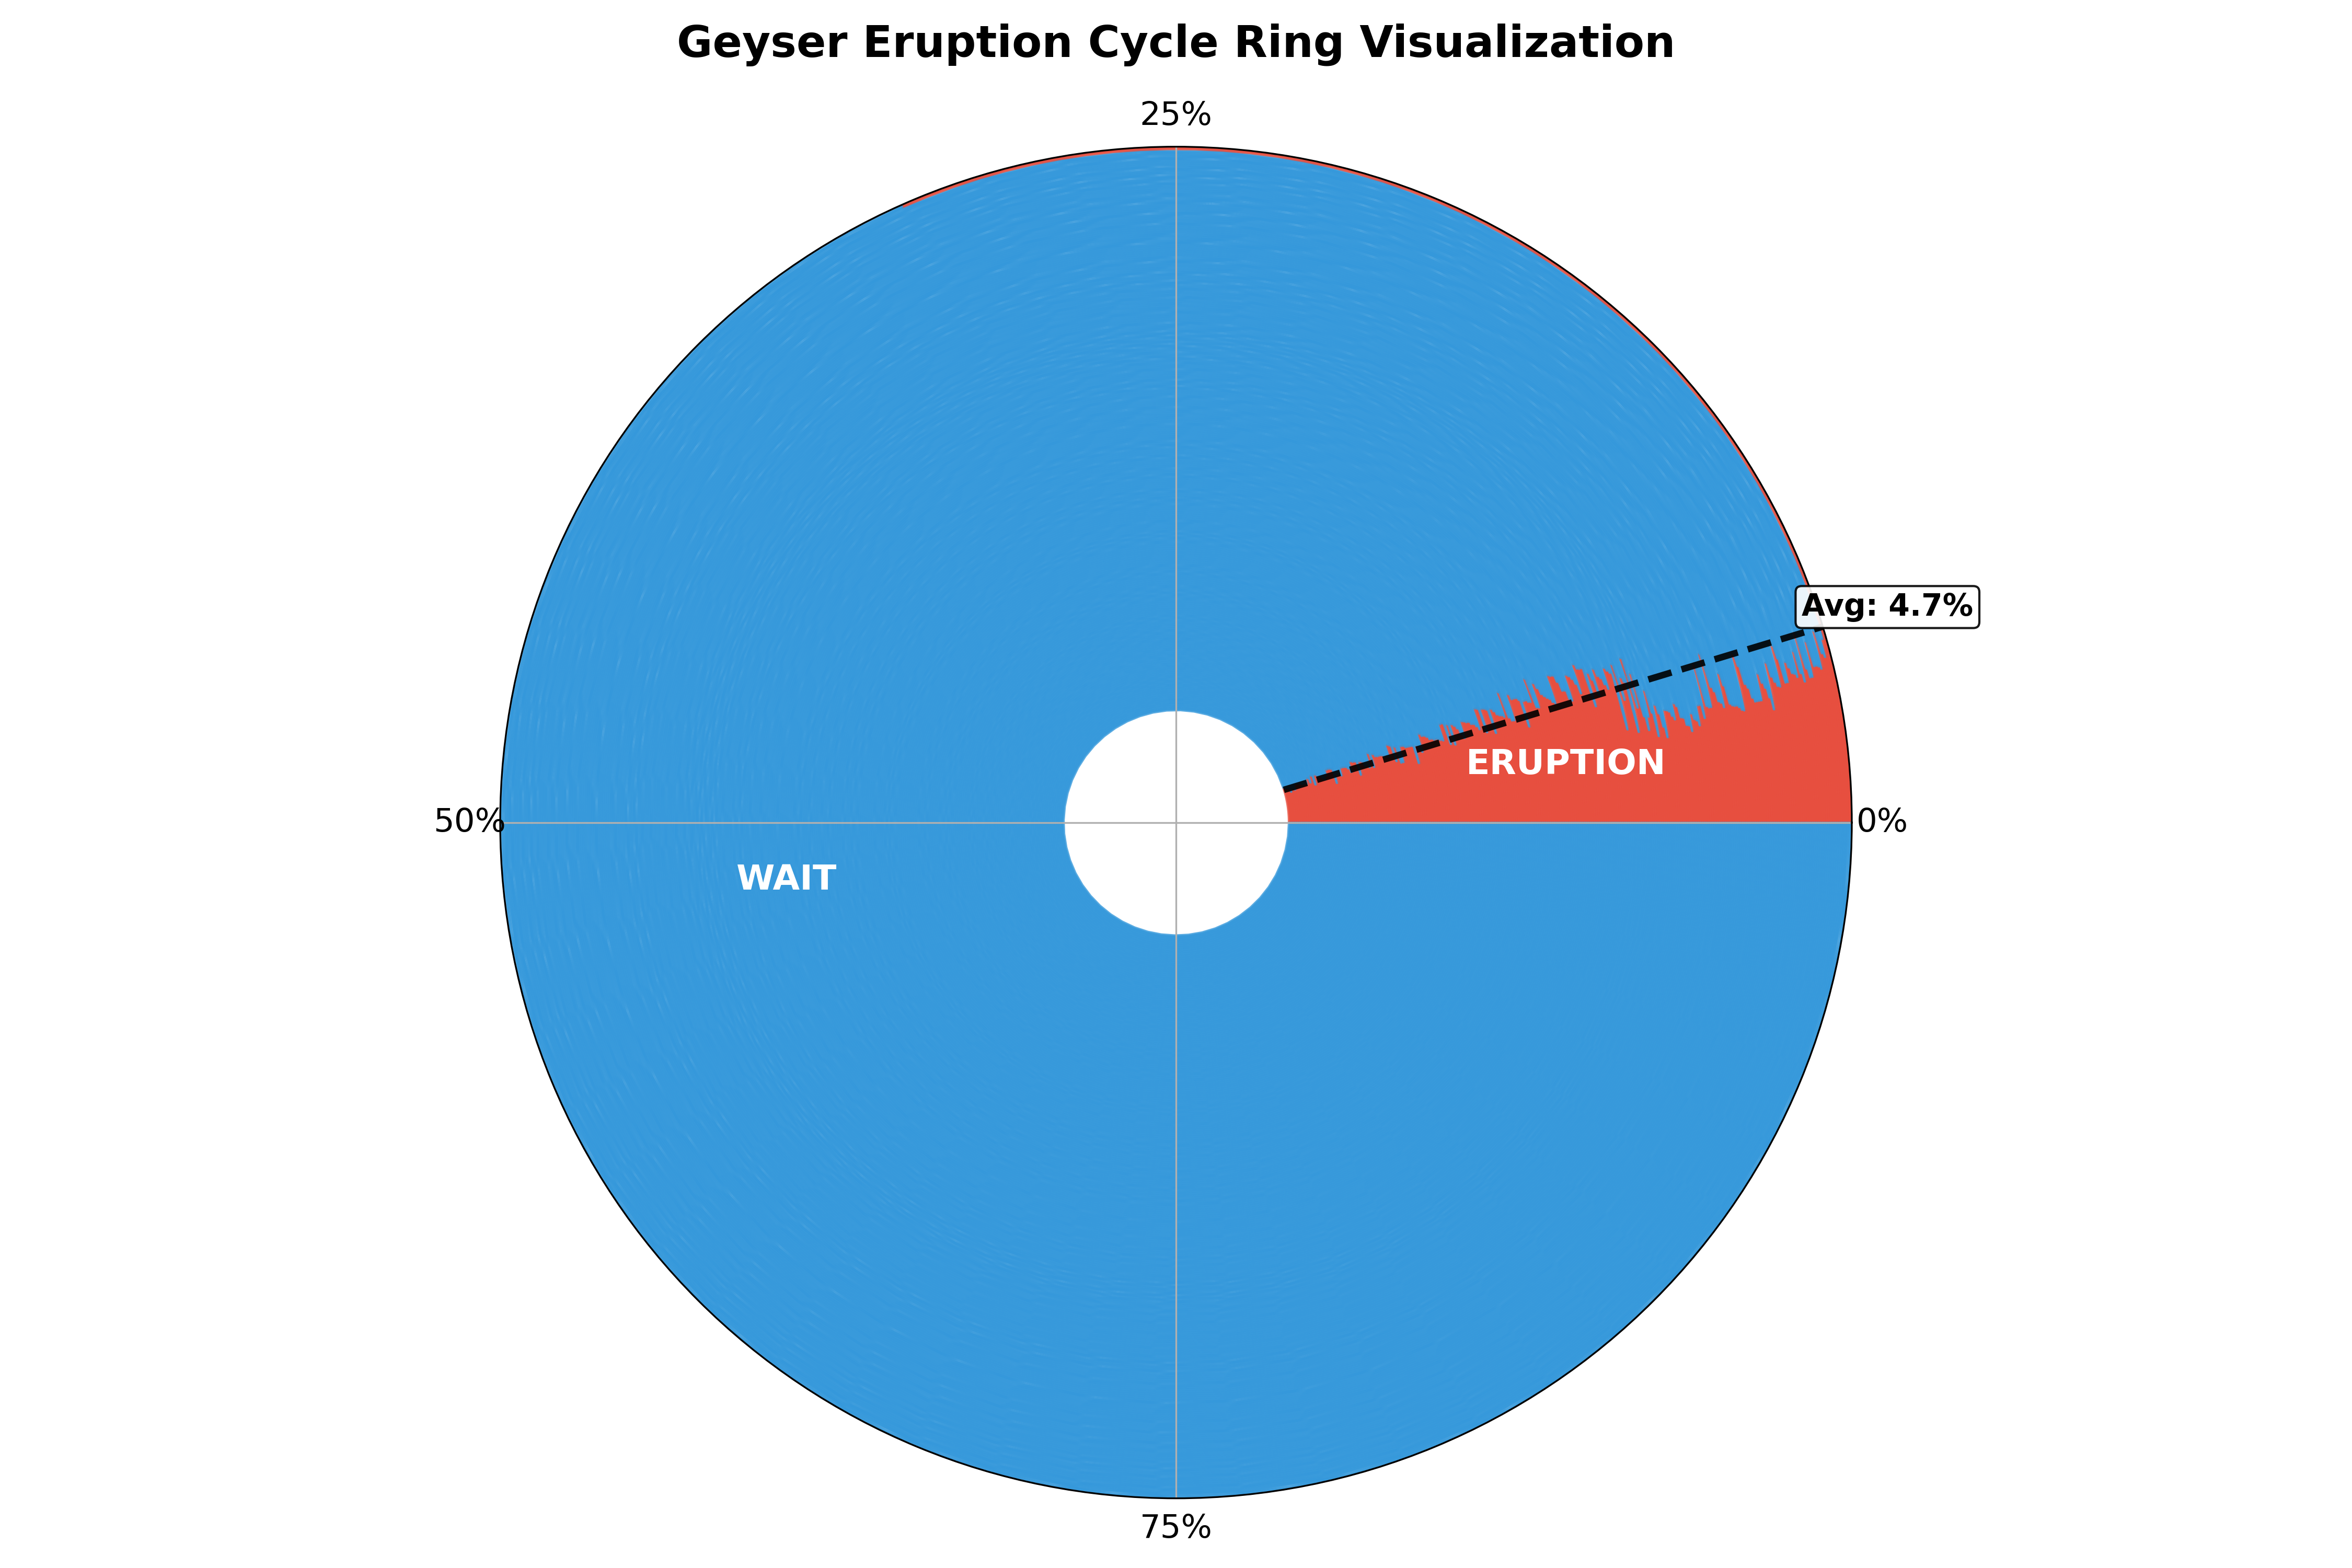
\includegraphics[width=0.8\linewidth]{pipeline_output/plots/periodicity_ring_analysis.png}
\caption{Ring visualization of Old Faithful geyser eruption cycles. Each ring represents one complete eruption cycle, with ring position indicating total cycle magnitude. Red arcs show eruption duration percentage, blue arcs show waiting time percentage. The dashed line indicates the average eruption duration percentage (35.8\%) across all cycles.}
\label{fig:periodicity}
\end{figure}

\section*{Discussion}

The preprocessing pipeline successfully addressed multiple data quality challenges while maintaining high data retention. The systematic approach to data cleaning ensures reproducibility and provides complete documentation of all modifications. The identification of alphanumeric contamination highlights the importance of data validation in scientific datasets, as such errors could significantly impact downstream analyses.

The ring visualization provides unique insights into geyser periodicity that traditional linear plots might obscure. The preservation of both magnitude and proportional information in a single visualization enables pattern recognition that could inform predictive models. The observed consistency in proportional relationships across different cycle magnitudes suggests underlying physical constraints that govern geyser behavior.

However, limitations exist in our approach. The logical constraint removing samples where eruption time exceeds waiting time, while physically reasonable, represents a subjective decision that could benefit from domain expert validation. Additionally, the ring visualization, while informative, may be less intuitive for readers unfamiliar with polar coordinate systems.

\section*{Conclusions}

This work demonstrates the effectiveness of systematic data preprocessing in preparing real-world datasets for analysis. Our pipeline achieved high data retention (98.2\%) while addressing multiple quality issues, establishing a framework applicable to similar temporal datasets. The novel ring visualization successfully reveals periodicity patterns in geyser behavior, showing consistent proportional relationships between eruption and waiting periods across different cycle magnitudes.

The developed methods provide a foundation for further investigation into geyser predictive modeling and offer a template for quality assessment in natural phenomena datasets. Future work could explore the application of these visualization techniques to other cyclical natural processes and investigate the physical mechanisms underlying the observed proportional consistency.

\section*{Acknowledgments}

The author thanks Prof. Matthew Reyna and the BMI 500 course staff for guidance on ethical data science practices and data visualization principles.

\end{document}
